% At least, use document class book
\documentclass[a4paper]{article}

\usepackage[T1]{fontenc}
\usepackage[latin1]{inputenc}
\usepackage{listings}
\usepackage{graphicx}
\usepackage{eso-pic}
\usepackage{pstricks}
\usepackage{listings}

\usepackage{color}
\definecolor{darkgreen}{rgb}{0,0.5,0}

% F�r listings
\usepackage{listings}
\lstset{
  frame=single,
  frameround=tttt,
  xleftmargin=0.7cm,
  xrightmargin=0.3cm,
  numbers=left,
  basicstyle=\fontfamily{pcr} \small \color{black},
  keywordstyle=\bfseries \color{blue},
	stringstyle=\color{red},
	commentstyle=\color{darkgreen},
	breaklines=true,
	showstringspaces=false
}

% F�r Metadaten im PDF.
\usepackage[
  bookmarksnumbered=true,
  pdftitle={How to use the OCL2 Interpreter},
  pdfauthor={Claas Wilke},
  pdfcreator={TeXnicCenter},
  pdfkeywords={OCL, Dresden OCL, constraints, interpretation},
  pdfsubject={A Tutorial which describes how the OCL2 Interpreter of Dresden OCL2 for Eclipse can be used.}
]{hyperref}
\definecolor{LinkColor}{rgb}{0,0,1}
	
\hypersetup{
  colorlinks=true,
  linkcolor=LinkColor,
  citecolor=LinkColor,
  filecolor=LinkColor,
  menucolor=LinkColor,
  urlcolor=LinkColor
} 

\newcommand{\reference}[1]{{\begin{ttfamily}#1\end{ttfamily}}}
\newcommand{\keyword}[1]{{\begin{itshape}#1\end{itshape}}}

\newcommand{\model}[1]{{\begin{ttfamily}#1\end{ttfamily}}}
\newcommand{\eclipse}[1]{{\begin{itshape}#1\end{itshape}}}


\begin{document}

% Define the title of the thesis
\title{How to use the OCL2 Interpreter}
% Specify the author of the thesis
\author{Claas Wilke}
% Specify the date on which the thesis is handed in

\maketitle

This tutorial describes how the OCL2 Interpreter provided with \keyword{Dresden OCL2 for Eclipse} can be used. A general introduction into \keyword{Dresden OCL2 for Eclipse} can be found in \cite{tut:general}. 

The procedure described in this tutorial was realized and tested with \keyword{Eclipse 3.4.1} \cite{WWW:Eclipse}. In addition to that this tutorial should also run with \keyword{Eclipse 3.3.x}. Besides \keyword{Eclipse} some required plug-ins must be installed. Table \ref{tab:software} shows all required software to run \keyword{Dresden OCL2 for Eclipse} and the OCL2 Interpreter.
  
\begin{figure}[!htbp]
\begin{tabular}[h]{|p{5.2cm}|p{6cm}|}
    \hline
    \textbf{Software} & \textbf{Available at} \\
    \hline
    Eclipse 3.4.x & http://www.eclipse.org/ \\
    \hline
    Eclipse Modeling Framework\newline (EMF) & http://www.eclipse.org/modeling/emf/ \\
    \hline
    Eclipse Model Development Tools\newline (MDT) (only with the UML2.0\newline meta model) & http://www.eclipse.org/modeling/mdt/ \\
    \hline
    Eclipse Plugin Development\newline Environment (only to run the\newline toolkit using the source code\newline distribution) & http://www.eclipse.org/pde/ \\
    \hline
\end{tabular}
\caption{Required software to run Dresden OCL2 for Eclipse and the OCL2 Interpreter.}
\label{tab:software}
\end{figure}


	
	
\section{How to Run Dresden OCL2 for Eclipse}

How to install and run \keyword{Dresden OCL2 for Eclipse} and how to load models and OCL constraints will not be explained in this tutorial. This tutorial assumes that the user is familiar with such basic uses of the toolkit. A general introduction into \keyword{Dresden OCL2 for Eclipse} can be found in \cite{tut:general}.




\section{The Simple Example}

This tutorial uses the \keyword{Simple Example} which is provided with \keyword{Dresden OCL2 for Eclipse} located in the plug-in package \reference{tudresden.ocl20.pivot.examples.\linebreak[0]simple}. An overview over all examples provided with \keyword{Dresden OCL2 for Eclipse} can be found in \cite{tut:examples}. Figure \ref{pic:Simple} shows the class structure which is described by the \keyword{Simple Example}. 

\begin{figure}[!htbp]
	\centering
	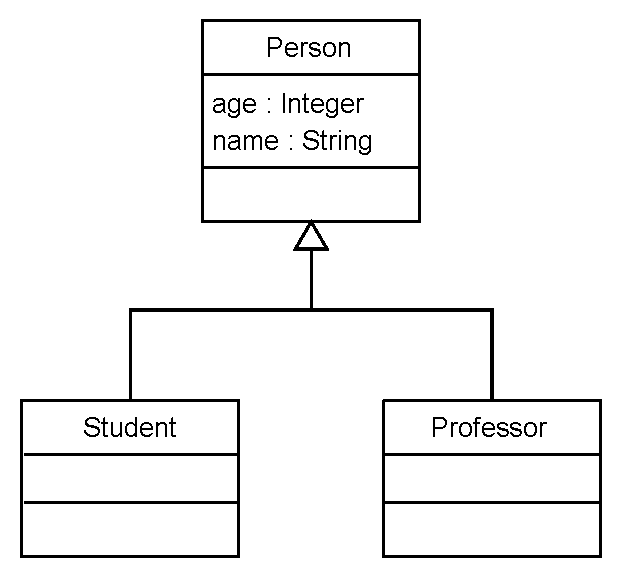
\includegraphics[width=0.5\linewidth]{../figures/simpleExample}
	\caption{The class structure described by the Simple Example model.}
	\label{pic:Simple}
\end{figure}

The model of the example defines three classes: The class \model{Person} has two attributes \model{age} and \model{name}. Two subclasses of \model{Person} are defined, \model{Student} and \model{Professor}.

To import the \keyword{Simple Example} into our Eclipse workspace we create a new Java project into our Workspace called \model{tudresden.ocl20.pivot.examples.\linebreak[0]simple} and use the import wizard \eclipse{General > Archive File} to import the example provided as jar archive. In the following window we select the directory were the jar file is located (eventually the \model{plugins} directory into the Eclipse root folder) and we select the archive \model{tudresden.ocl20.pivot.examples.simple.\linebreak[0]jar} and click the \eclipse{Finish} button (if you use a source code distribution of \keyword{Dresden OCL2 for Eclipse} instead, you can simple import the project \model{tudresden.ocl20.\linebreak[0]pivot.examples.simple} using the import wizard \eclipse{General -> Existing Projects into Workspace}). Figure \ref{pic:packageExplorer} shows the package Explorer containing the imported project.

\begin{figure}[!htbp]
	\centering
	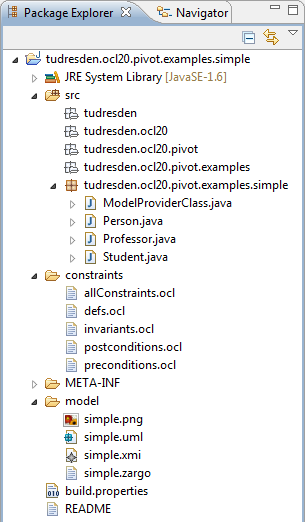
\includegraphics[width=0.6\linewidth]{figures/packageExplorer}
	\caption{The package explorer containing the project which is needed to run this tutorial.}
	\label{pic:packageExplorer}
\end{figure}

The project provides a model file which contains the simple class diagram (the model file is located at \model{model/simple.uml}) and the constraint file we want to interpret (located at \model{constraints/allConstraints.ocl}). Listing \ref{lst:allConstraints} shows the constraints defined in the constraint file.

\lstset{
  language=OCL
}
\begin{lstlisting}[caption={The constraints contained in the constraint file.}, captionpos=b, label=lst:allConstraints, float]
-- The age of Person can not be negative.
context Person
inv: age >= 0

-- Students should be 16 or older.
context Student
inv: age > 16

-- Proffesors should be at least 30.
context Professor
inv: not (age < 30)

-- Returns the age of a Person.
context Person
def: getAge(): Integer = age

-- Before returning the age, the age must be defined.
context Person::getAge()
pre: not age.oclIsUndefined()

-- The result of getAge must equal to the age of a Person.
context Person::getAge()
post: result = age
\end{lstlisting}

First, the constraint file defines three simple invariants which denote, that the \model{age} of every \model{Person} must always zero or greater than zero. Furthermore, the \model{age} of every \model{Student} must be greater than 16 and the  \model{age} of every \model{Professor} does not have to be lesser than 30.

In addition to that the constraint file contains a definition constraint which defines a new operation \model{getAge()} which returns the \model{age} of a \model{Person}. A precondition checks, that the \model{age} must be defined before it can be returned by the operation \model{getAge()}. And finally, a postcondition checks, whether or not the result of the operation \model{getAge()} is the same as the \model{age} of the \model{Person}.




\section{Preparation of the Interpretation}

To prepare the interpretation we have to import the model \model{model/simple.uml} for which we want to interpret constraints into the \eclipse{Model Browser}. We use the import wizard for domain specific models of the toolkit to import the model. This procedure is explained in the already mentioned general tutorial (\cite{tut:general}). Furthermore, we have to import a model instance for which the constraints shall be interpreted into the \eclipse{Model Instance Browser}. We use another import wizard to import the model instance \model{bin/tudresden/ocl20/pivot/examples/simple\linebreak[0]/\linebreak[0]ModelProviderClass.class}. Finally, we have to import the constraint file \model{constraints/allConstraints.ocl} containing the constraints we want to interpret. The import is done by an import wizard again. Afterwards, the \eclipse{Model Browser} should look like illustrated in figure \ref{pic:modelBrowser} and the \eclipse{Model Instance Browser} should look like shown in figure \ref{pic:modelInstanceBrowser}.

\begin{figure}[!htbp]
	\centering
	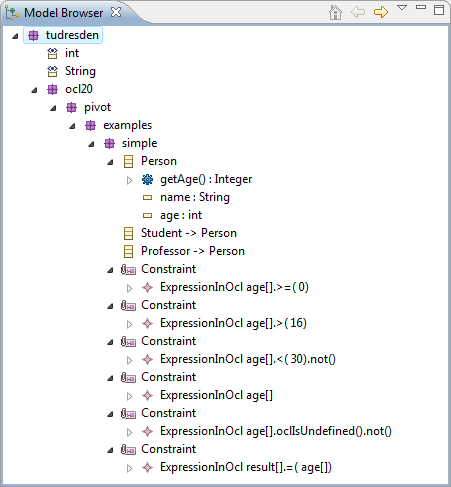
\includegraphics[width=0.8\linewidth]{figures/modelBrowser}
	\caption{The model browser containing the simple model and its constraints.}
	\label{pic:modelBrowser}
\end{figure}

\begin{figure}[!htbp]
	\centering
	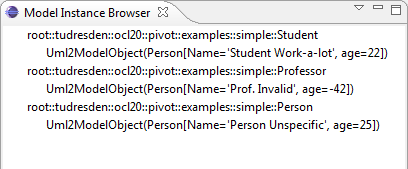
\includegraphics[width=0.7\linewidth]{figures/modelInstanceBrowser}
	\caption{The model instance browser containing the simple model instance.}
	\label{pic:modelInstanceBrowser}
\end{figure}

The loaded model instance contains three instances of the classes defined in the \keyword{Simple Example} model. One instance of \model{Person}, one instance of \model{Student} and one instance of \model{Professor}. For these three instances we now want to interpret the imported constraints.




\section{Interpretation}

Now we can start the interpretation. To open the \keyword{OCL2 Interpreter} we use the menu option \reference{Dresden OCL2 > Open OCL2 Interpreter}. The \eclipse{OCL2 Interpreter View} should now be visible (see figure \ref{pic:interpreter01}).

\begin{figure}[!htbp]
	\centering
	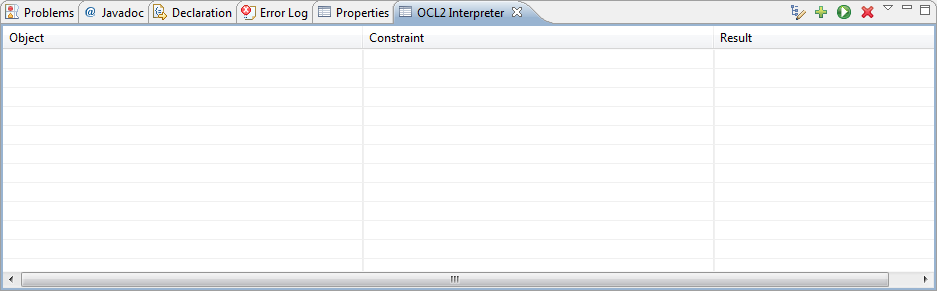
\includegraphics[width=1.0\linewidth]{figures/interpreter01}
	\caption{The OCL2 Interpreter containing no results.}
	\label{pic:interpreter01}
\end{figure}

By now, the \eclipse{OCL2 Interpreter View} does not contain any result. Besides the results table, the view provides four buttons to control the \keyword{OCL2 Interpreter}. The buttons are shown in figure \ref{pic:interpreter02}. With the first button (from left to right) constraints can be prepared for interpretation. The second button can be used to add variables to the \keyword{Interpreter Environment}. The third button provides the core functionality, it can be used to start the interpretation. And finally, the fourth button provides the possibility to delete all results from the \eclipse{OCL2 Interpreter View}. The functionality of the buttons will be explained below.

\begin{figure}[!htbp]
	\centering
	
\includegraphics[width=0.5\linewidth]{figures/interpreter02}
	\caption{The buttons to control the OCL2 Interpreter.}
	\label{pic:interpreter02}
\end{figure}


\subsection{Interpretation of Constraints}

To interpret constraints, we simple select them in the \eclipse{Model Browser} and press the button to interpret constraints (the third button from the left). First, we want to interpret the three invariants defining the range of the \model{age} of \model{Persons}, \model{Students} and \model{Professors}. We select them in the \eclipse{Model Browser} (see figure \ref{pic:interpreter03}) and click the \eclipse{Interpret} button. The result of the interpretation is now shown in the \eclipse{OCL2 Interpreter View} (see figure \ref{pic:interpreter04}).

\begin{figure}[!htbp]
	\centering
	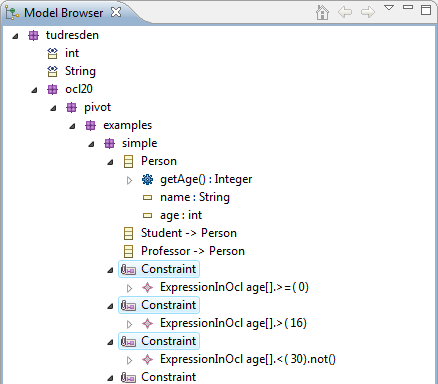
\includegraphics[width=0.7\linewidth]{figures/interpreter03}
	\caption{The three age invariants selected in the Model Browser.}
	\label{pic:interpreter03}
\end{figure}

\begin{figure}[!htbp]
	\centering
	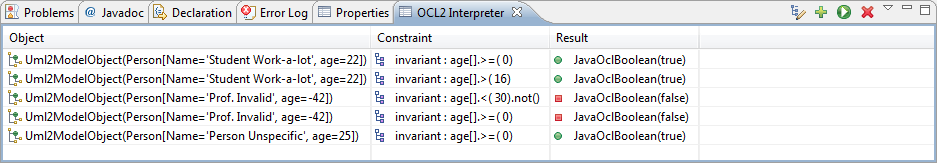
\includegraphics[width=1.0\linewidth]{figures/interpreter04}
	\caption{The results of the three age invariants for all model instances.}
	\label{pic:interpreter04}
\end{figure}

The invariant \model{age >= 0} has been interpreted for all three model objects. The results for the \model{Person} and the \model{Student} instances are \model{true} because their \model{age} is greater than zero. The result for the \model{Professor} instance is \model{false} because its \model{age} is \model{-42}.

The two other invariants were only interpreted for the \model{Student} or the \model{Pro\-fessor} instance because their context was not the class \model{Person} but the class \model{Student} or the class \model{Professor}. Again the \model{Student's} result is \model{true} and the \model{Professor's} result is \model{false}.


\subsection{Preparation of Constraints}

Some constraints cannot be interpreted because they are no constraints in the natural sense of the word constraint. OCL enables us to use constraints to define new attributes and methods or to initialize attributes and methods. Such \model{def}, \model{init} and \model{body} constraints cannot be interpreted because they have no result. They can only be used to alter the results of other constraints which shall be interpreted.

The \keyword{Simple Example} constraint file contains a definition constraint, which defines the method \model{getAge()} for the class \model{Person}. Before we can refer to this method in other constraints we have to prepare the definition constraint to ensure, that the interpretation of other constraints will finish with the right results.

To prepare the definition constraint, we select it in the \eclipse{Model Browser} (see figure \ref{pic:interpreter05}) and click the \eclipse{Prepare} button (the first button from the left).

\begin{figure}[!htbp]
	\centering
	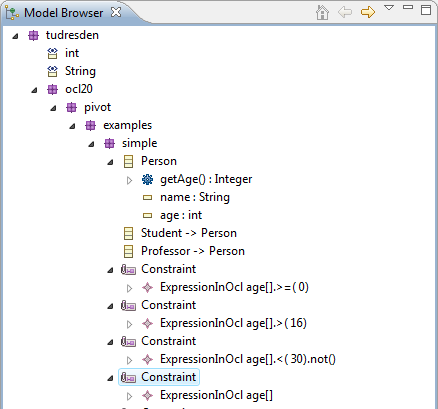
\includegraphics[width=0.7\linewidth]{figures/interpreter05}
	\caption{The definition constraint selected in the Model Browser.}
	\label{pic:interpreter05}
\end{figure}

The preparation does not result with a visible result in the \eclipse{OCL2 Interpreter View}. But the method definition of the constraint has been added to the \keyword{Interpreter Environment} of the \keyword{OCL2 Interpreter}. Thus, we can interpret the next constraint now. This constraint is the precondition which checks that the \model{age} of any \model{Person} must be defined before the method \model{getAge()} can be invoked.

We select the constraint in the \eclipse{Model Browser} (see figure \ref{pic:interpreter06}) and click the \eclipse{Interpret} button. The result of the interpretation is shown in figure \ref{pic:interpreter07}.

\begin{figure}[!htbp]
	\centering
	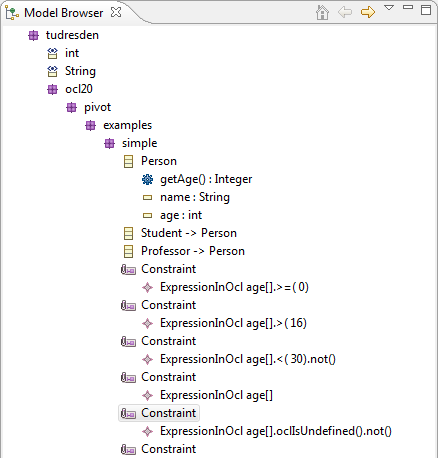
\includegraphics[width=0.7\linewidth]{figures/interpreter06}
	\caption{The precondition selected in the Model Browser.}
	\label{pic:interpreter06}
\end{figure}

\begin{figure}[!htbp]
	\centering
	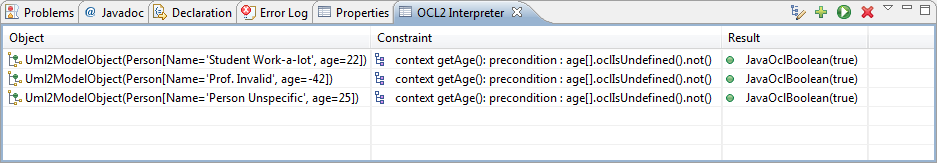
\includegraphics[width=1.0\linewidth]{figures/interpreter07}
	\caption{The results of the precondition for all model instances.}
	\label{pic:interpreter07}
\end{figure}

The interpretation finishes for all three instances successfully because the attribute \model{age} has been set for all three instances.


\subsection{Adding Variables to the Environment}

By preparing the definition constraint we added some information to the \keyword{Interpretation Environment} which was necessary to interpret other constraints. For some constraints we have to add further information which can not be provided by the preparation of other constraints.

For example, our last constraint a postcondition compares the result of the method \model{getAge()} with the attribute \model{age} of the referenced \model{Person} instance. Therefore, OCL provides the special variable \model{result} in postconditions which contains the result of the constrained method's execution. Using the \eclipse{OCL2 Interpreter View} we cannot execute the method \model{getAge()} and store the result in the \model{result} variable. We can interpret the postcondition in a specific context which has to be prepared by hand only. We have to set the result variable manually.

If we interpret the postcondition constraint (the sixth and last constraint in the \eclipse{Model Browser}) without setting the \model{result} variable, the constraint results in a \model{undefined} result for all three model instances (see figure \ref{pic:interpreter08}).

\begin{figure}[!htbp]
	\centering
	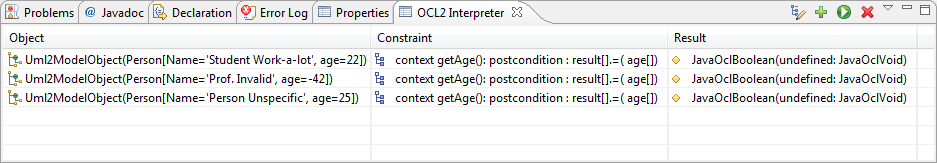
\includegraphics[width=1.0\linewidth]{figures/interpreter08}
	\caption{The results of the postcondition without preparing the result variable.}
	\label{pic:interpreter08}
\end{figure}

To prepare the variable we click on the button to add new variables to the \keyword{Interpreter Environment} (the second button from the left) and a new window opens which we can use to specify new variables. We enter the name \model{result}, select the variable type \model{Integer} and enter the value \model{25}. Then we press the \eclipse{OK} button (see figure ref{pic:interpreter09}. The result variable has now been added to the \keyword{Interpreter Environment}.

\begin{figure}[!htbp]
	\centering
	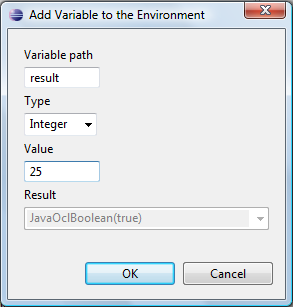
\includegraphics[width=0.5\linewidth]{figures/interpreter09}
	\caption{The window to add new variables to the environment.}
	\label{pic:interpreter09}
\end{figure}

\begin{figure}[!htbp]
	\centering
	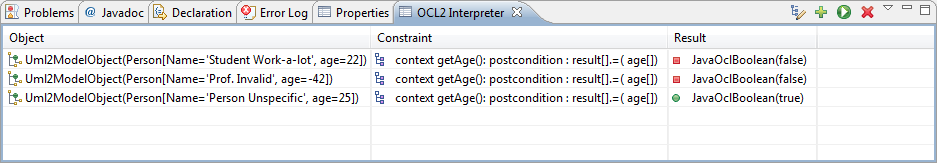
\includegraphics[width=1.0\linewidth]{figures/interpreter10}
	\caption{The results of the postcondition with result variable preparation.}
	\label{pic:interpreter10}
\end{figure}

Now we can interpret the postcondition again. The result is shown in figure \ref{pic:interpreter10}. The results for the \model{Student} and \model{Professor} instances are both \model{false} because their \model{age} attribute is not equal to \model{25} and thus the \model{result} value does not match to the \model{age} attribute. But the interpretation for the \model{Person} instances succeeds because its age is \model{25}.




\section{Conclusion}
  
This tutorial described how OCL2 constraints can be interpreted using the \textit{OCL2 Interpreter} of \textit{Dresden OCL2 for Eclipse}. The preparation and interpretation of constraints has been explained, the addition of new variables to the \keyword{Interpreter Environment} has been shown.

More information about \textit{Dresden OCL2 for Eclipse} can be found at \cite{WWW:toolkit}.




\newpage
\bibliographystyle{alphadin}
\bibliography{interpreter}
% Literaturliste in Inhalt aufnehmen.
\addcontentsline{toc}{section}{References}




\end{document}
